\documentclass[12pt]{article}
\setlength{\oddsidemargin}{0in}
\setlength{\evensidemargin}{0in}
\setlength{\textwidth}{6.5in}
\setlength{\parindent}{0in}
\setlength{\parskip}{\baselineskip}
\usepackage{amsmath,amsfonts,amssymb}
\usepackage{graphicx}
\usepackage{mathtools}
\usepackage{color}
\usepackage{fancyhdr}
\pagestyle{fancy}
%----------------------------------------------------------------------------
\begin{document}
\lhead{{\bf CSCI 3753 \\ Problem Set 1} }
\rhead{{\bf Liam Kolber\\ Spring 2018, CU-Boulder}}
\renewcommand{\headrulewidth}{0.4pt}
\begin{enumerate}
%----------------------------------------------------------------------------
	\item \textit{What are the three high level features that are provided by an Operating System?}
		\begin{enumerate}
			\item \underline{Hardware Abstraction:} The OS controls use of hardware components among all of the applications and provides an easy link to communicating to said hardware so individual applications don't need to be aware of specific hardware details.
			\item \underline{Resource Management:} The OS controls the access and division of computer resources (i.e. CPU) in order to maintain efficiency as well as speed. This prevents a single application from hogging everything and putting other (sometimes quick and efficient) processes from getting CPU time.
			\item \underline{Protection:} The OS protects the system and its components by isolating processes. This protects applications and programs from affecting each other (unless intended) as well as limiting resource consumption to prevent one application from hogging it all and to prevent damage to components. Lastly, it also protects the OS from the user and applications unless specifically intended.
	    \end{enumerate}
%----------------------------------------------------------------------------
	\item \textit{Why does an Operating System need protection from user code?} \\
	The OS and user code share computer hardware in order to run. If a bug in user-written code prevents other processes or programs from executing properly, then the risk of damage or file corruption increases. OS's typically have multiple modes (i.e. user mode and kernel mode) that protect key processes when the user isn't intending to alter those processes.
%----------------------------------------------------------------------------
	\item \textit{What are the four major components of an Operating System?}
		\begin{enumerate}
			\item \underline{File Manager:} \\
			The file manager handles the abstraction and organization of files on the system as well as reading from and writing to said files. It also helps in the search and listing of files for the user to easily interact with.
			\item \underline{Memory Manager:} \\
			The memory manager is responsible for keeping and organizing as many currently working process and information in memory as possible to increase the efficiency of the CPU. It is also responsible for deciding when and which process have access to certain sections of memory at any given time.
			\item \underline{Process Manager:} \\
			Also known as the scheduler, this components is responsible for organizing queued processes in order to (ideally) be as efficient as possible to ensure quick resolutions to all queued processes. 
			\item \underline{Device Manager:} \\
			The device manager handles interactions with all devices connected to the system to ensure proper communication between components as well as communication between the user and the system.
		\end{enumerate}
%----------------------------------------------------------------------------
	\item \textit{How does a user application system code within the Operating System?}\\
	User applications are able to code within the OS by the use of the \verb|trap| instruction. It works by toggling the mode bit to $0$ (entering Kernel Mode) and is referred to as a system call. When the system call ends,
%----------------------------------------------------------------------------
	\item \textit{How are parameters passed to and results returned from a System Call?}\\
	Parameters are passed to a System Call via a System Interrupt. The kernel then checks what interrupt has been made in order to see what system call is occurring. Any additional information is passed in registers or in memory, and once the kernel verifies the request and executes, the kernel flips the mode back from kernel mode and continues with the next instruction.
%----------------------------------------------------------------------------
	\item \textit{What are the steps taken to start up a computer?}\\
	The very first thing to happen when a computer starts is a predetermined set of basic diagnostics in order to ensure that all necessary components are connected and functioning properly. The bios is then loaded which allows for enough control to communicate with the boot device carrying the Bootstrap program. The Bootstrap program then locates the OS, loads it into memory, and begins the process of starting up the OS.
%----------------------------------------------------------------------------
	\item \textit{What is a Virtual Machine and how does it differ from a physical machine?}\\
	A virtual machine is a fully functioning operating system that operates on top of an already functioning OS. The benefit of these VM's is the fact that the user can save states of the VM allowing the user to tweak the OS without the fear of permanent damage. The major difference between a VM and traditional OS is in the structure. In a VM, an extra layer between the kernel of the host machine and the OS of the VM exists known as the "hypervisor." This layer exists to create multiple identical environments and allows for the management of the guest OS and any guest processes.
%----------------------------------------------------------------------------
\newpage
	\item \textit{Describe the difference between multi-programming and multi-tasking?}\\
	Multi programming is when CPU runs a certain program until it hits a "lightweight" stage (i.e. writing to a file) and begins running the next program in the queue. This can be tricky because an infinite loop could prevent further computations until it's resolved.\\
	Multi-tasking is when the cpu is constantly switching between a set of programs in the queue at equal intervals. This maximizes efficiency as the CPU never has down time in the case of an unintentional infinite loop or something of the sort.
%----------------------------------------------------------------------------
	\item \textit{What is a context switch?}\\
	A context switch is the concept of switching between programs. In order to do so, there is about $1\mu s$ of time in which the CPU need to save the state of the current program to not lose progress. This is called the context switch overhead.
%----------------------------------------------------------------------------
	\item \textit{Provide a timing chart for the processes listed below using multi-programming and another when using multi-tasking.}
		\begin{center}
			\begin{tabular}{ |c|c|c|c| } 
				\hline
				Process & Length & Arrival Time & IO (time,wait) \\ 
				\hline\hline
				P1 & 40 & 0 & (20,30) \\ 
				\hline
				P2 & 20 & 10 & none \\
				\hline
				P3 & 25 & 30 & none \\
				\hline
			\end{tabular}
			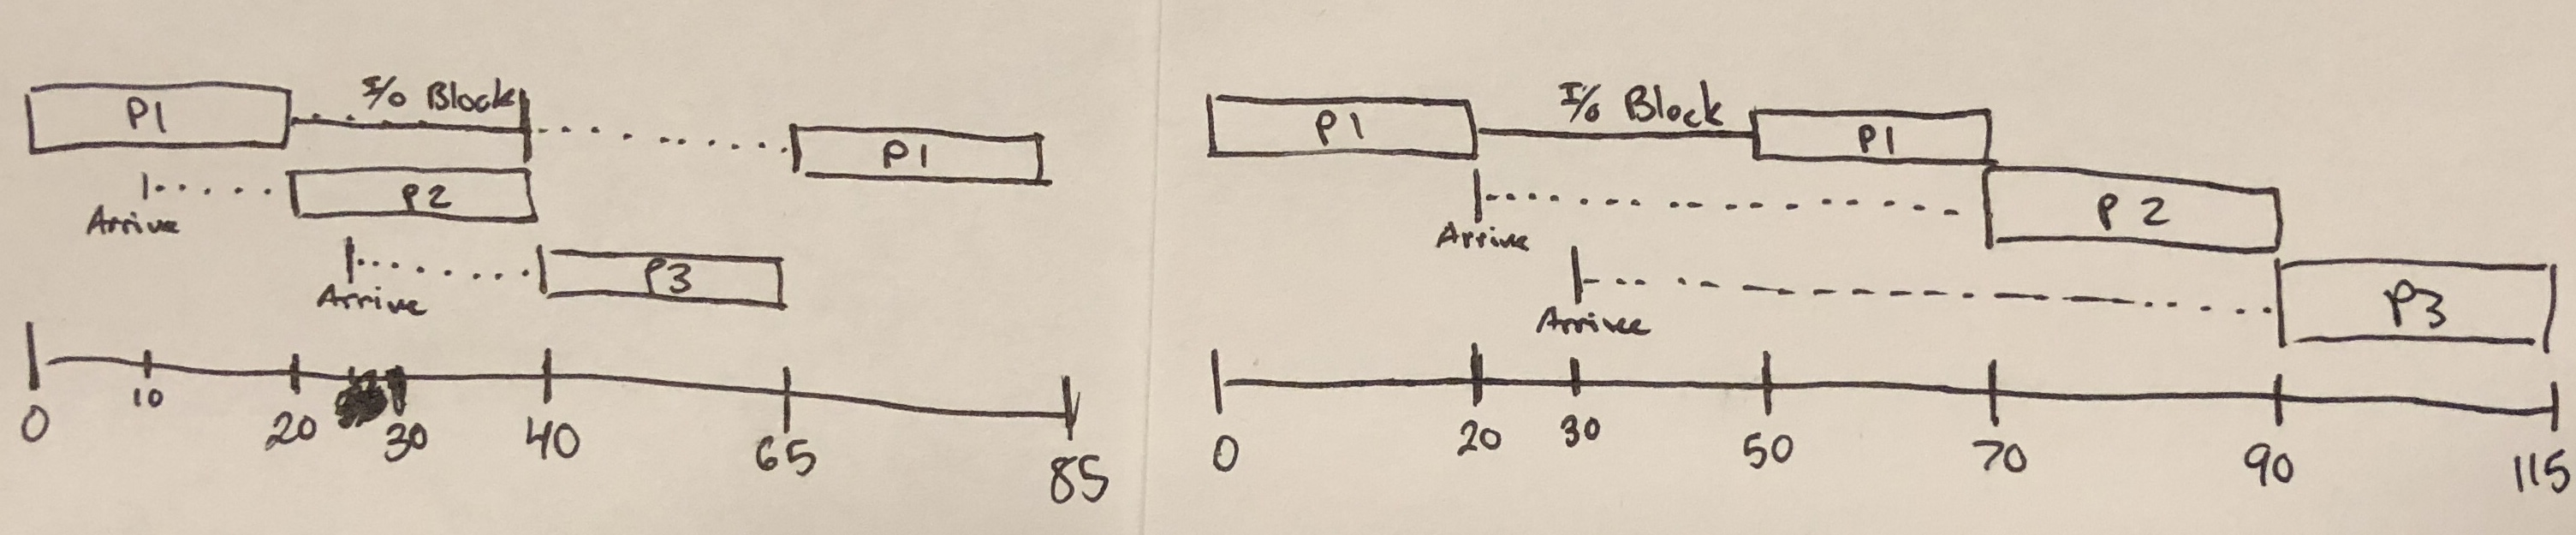
\includegraphics[width=\textwidth]{IMG_0334.jpg}
		\end{center}
\end{enumerate}
\end{document}
%----------------------------------------------------------------------------